\section{System Overview}

The BPM system can be broadly divided into three components (as shown in Figure \ref{fig:sys_overview}). The first component is the client Android application. It is the core component of the BPM system, which provides an interface allowing users to register with our system. In addition, the application also allows users to easily look up available parking lots and buy permits for desired parking lots. Another main task of the Android application is scanning available Bluetooth devices around the user. It periodically scans a discoverable Bluetooth device which is attached to the gate of parking lot or garage. 

\begin{figure}[ht]
	\centering
		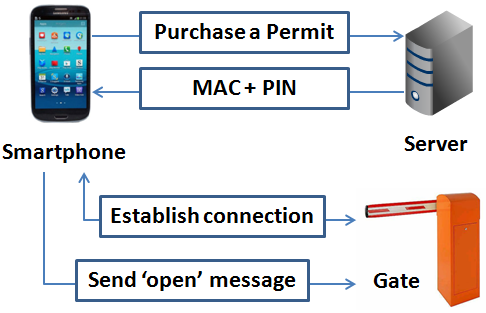
\includegraphics[width=3in]{figure/sys_overview.png}
		\caption{The BPM system consists of three components: client Android application, server, and Bluetooth enabled parking lot gate}
	\label{fig:sys_overview}
\end{figure}

The second component is the application server, which provides RESTful end-points for useful functions that are used by the client Android application. These functions include registration, parking lot searching, buying parking lot permits, etc. When a user registers with our system, he/she may search for parking lots simply buy providing a ZIP code, which then the server retrieves available parking lots and garages for the user. Oncec the user purchases the permit, the server returns the MAC address of the particular parking lot's Bluetooth device and the PIN associated with the Bluetooth device for pairing to establish a communication channel between the user's smartphone and the Bluetooth device.

The last component is the Bluetooth device which is attached to the gate of parking lot. It is essentially a combination of an Arduino board and a Bluetooth module. Once the user purchases the permit, the user's smartphone maintains the MAC address and the PIN. Once the client Android application finds the correct Bluetooth device by matching with the MAC address, it automatically initiates pairing process and establishes a communication channel. Once the communication channel is successfully established, the client Android application sends a message to the parking lot Bluetooth device to open the gate. The parking lot Bluetooth receives the message and command the gate to open via the Arduino board attached to the gate.